\scanpage{20}
\uline{NB} C'est une relation \deleted{d'ordre} \inserted{de préordre}. La relation d'équ. associée est $f'\sim f$.
\margin{\uline{NB} Le sup de $\langle f',g\rangle$ pour $f'\prec f$ est atteint \deleted{pour} \inserted{des} $f'\sim f\ldots$}

\deleted{\uline{Cor} $f'\prec f$, $g'\prec g\Longrightarrow|f',g'|\leq|f,g|$}

\uline{Cor} $f'\prec f\Longleftrightarrow\forall g',g\in C(G)^+$, avec $g'\prec g$, on a
\[
|f',g'|\leq|f,g|
\]

\uline{3}\quad\uline{Couples \unsure{pritorisés|priorisés}}

A partir de maintenant, $G$ est un groupe, d'où opération $f\ast g$ sur $\mathbb R[G]^{\unsure{\ast|+}}$, $\mathbb R[G]^+$ est stable.

\margin{\uline{NB} Soient $f,g\in\mathbb R(G)^+$. Considérons les $\|f'\ast g\|_\infty$ ou $(f'\ast g)(0)$ pour $f'\prec f$, alors le Sup est \deleted{\unsure{atteint}\ $\unsure{\|f\ast g\|_\infty}$} \inserted{$=$}, et il est atteint pour $f'\sim f$.}

\uline{Prop} $f,g\in\mathbb R(G)^+$, Conditions équivalentes

a) $f'\prec f$, $g'\prec g$, $\|f'\ast g'\|_\infty\leq\|f\ast g\|_\infty$

b) $\forall f'\prec f$, $g'\prec g$
\[
\underset{\inserted{=\langle f',\check g'\rangle}}{(f'\ast g')(0)}
\leq\operatorname{Sup}_{s\in G}
\underbrace{(f\ast g)(s)}_{\inserted{=\deleted{\unsure{\langle f,\check g\rangle}}\langle f\unsure{\ast|,}\varepsilon_s\check g\rangle}}
\]
a') \deleted{$\unsure{\forall f'\sim f,\ \forall g'\sim g}$} a), b) avec $f'\sim f$, $g'\sim g$

c) $|f,g|=\|f\ast g\|_\infty$

d) $\exists s\in G$ tel que
\diagram{\begin{tikzcd}[row sep=small]
\inserted{E_\ast(g)\cup E_\ast(\check f\ast\varepsilon_s)\ \deleted{\unsure{E_\ast(\check g)}}\ \text{tot. ordonné}}\arrow[d,leftrightarrow]\\
E_\ast(f)\cup E_\ast(\varepsilon_s\check g)\quad\text{tot. ordonné}
\end{tikzcd}}
i.e. $\forall\alpha,\beta\in\mathbb R^{+\ast}$, $E_\alpha(f)$ et $E_\beta(\varepsilon_s\check g)$ en relation d'inclusion

\uline{Def} On dit alors que le \deleted{\unsure{bi}}couple $(f,g)$ est \uline{\unsure{pritorisé|priorisé}}
([Il n'est pas clair que la relation soit symétrique --- \deleted{\unsure{elle signifie}\ $\forall s$} mais OK si $G$ commutatif])

\uline{Cor} $f\in\mathbb R[G]^+$, \deleted{\unsure{alors}} $(f,f)$ est \unsure{pritorisé|priorisé} (\deleted{\unsure{sss}\ $f\text{ et }f$} \inserted{$\exists s\in G$} tel que $\check f=\varepsilon_s\ast f$ ($\Longleftrightarrow\check f=f\ast\varepsilon_s$)

\margin{\figure{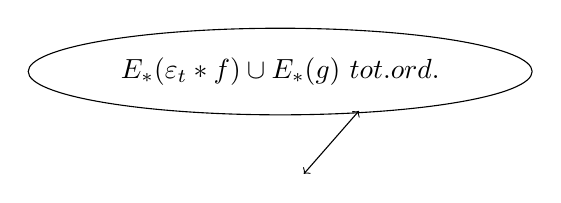
\begin{tikzpicture}[x=1cm,y=1cm]
\node at (0,0) {$E_\ast(\varepsilon_t\ast f)\cup E_\ast(g)\ \text{tot. ord.}$};
\draw (0,0) ellipse (3.2cm and .55cm);
\draw[<->] (1,-.5) -- (.3,-1.3);
\end{tikzpicture}}}
\uline{NB} Si dans la prop. $g$ satisfait la condition précédente, alors la condition de la prop signifie aussi \unsure{eq} $\exists t\in G$ t.q. $E_\ast(f)\cup E_\ast(\varepsilon_t\ast g)$ tot. ordonné
% archive foliation: 19
